\documentclass{article}

\usepackage{graphicx}
\usepackage{tikz}
\usepackage{tikzsymbols}
\usetikzlibrary{calc,patterns,shapes.geometric}
\pagestyle{empty}
\usepackage[margin=0pt]{geometry}
\geometry{papersize={14in,12in}}

\def\centerarc[#1](#2)(#3:#4:#5){\draw[#1] ($(#2)+({#5*cos(#3)},{#5*sin(#3)})$) arc (#3:#4:#5);}

\begin{document}
	\begin{figure}
		\centering
		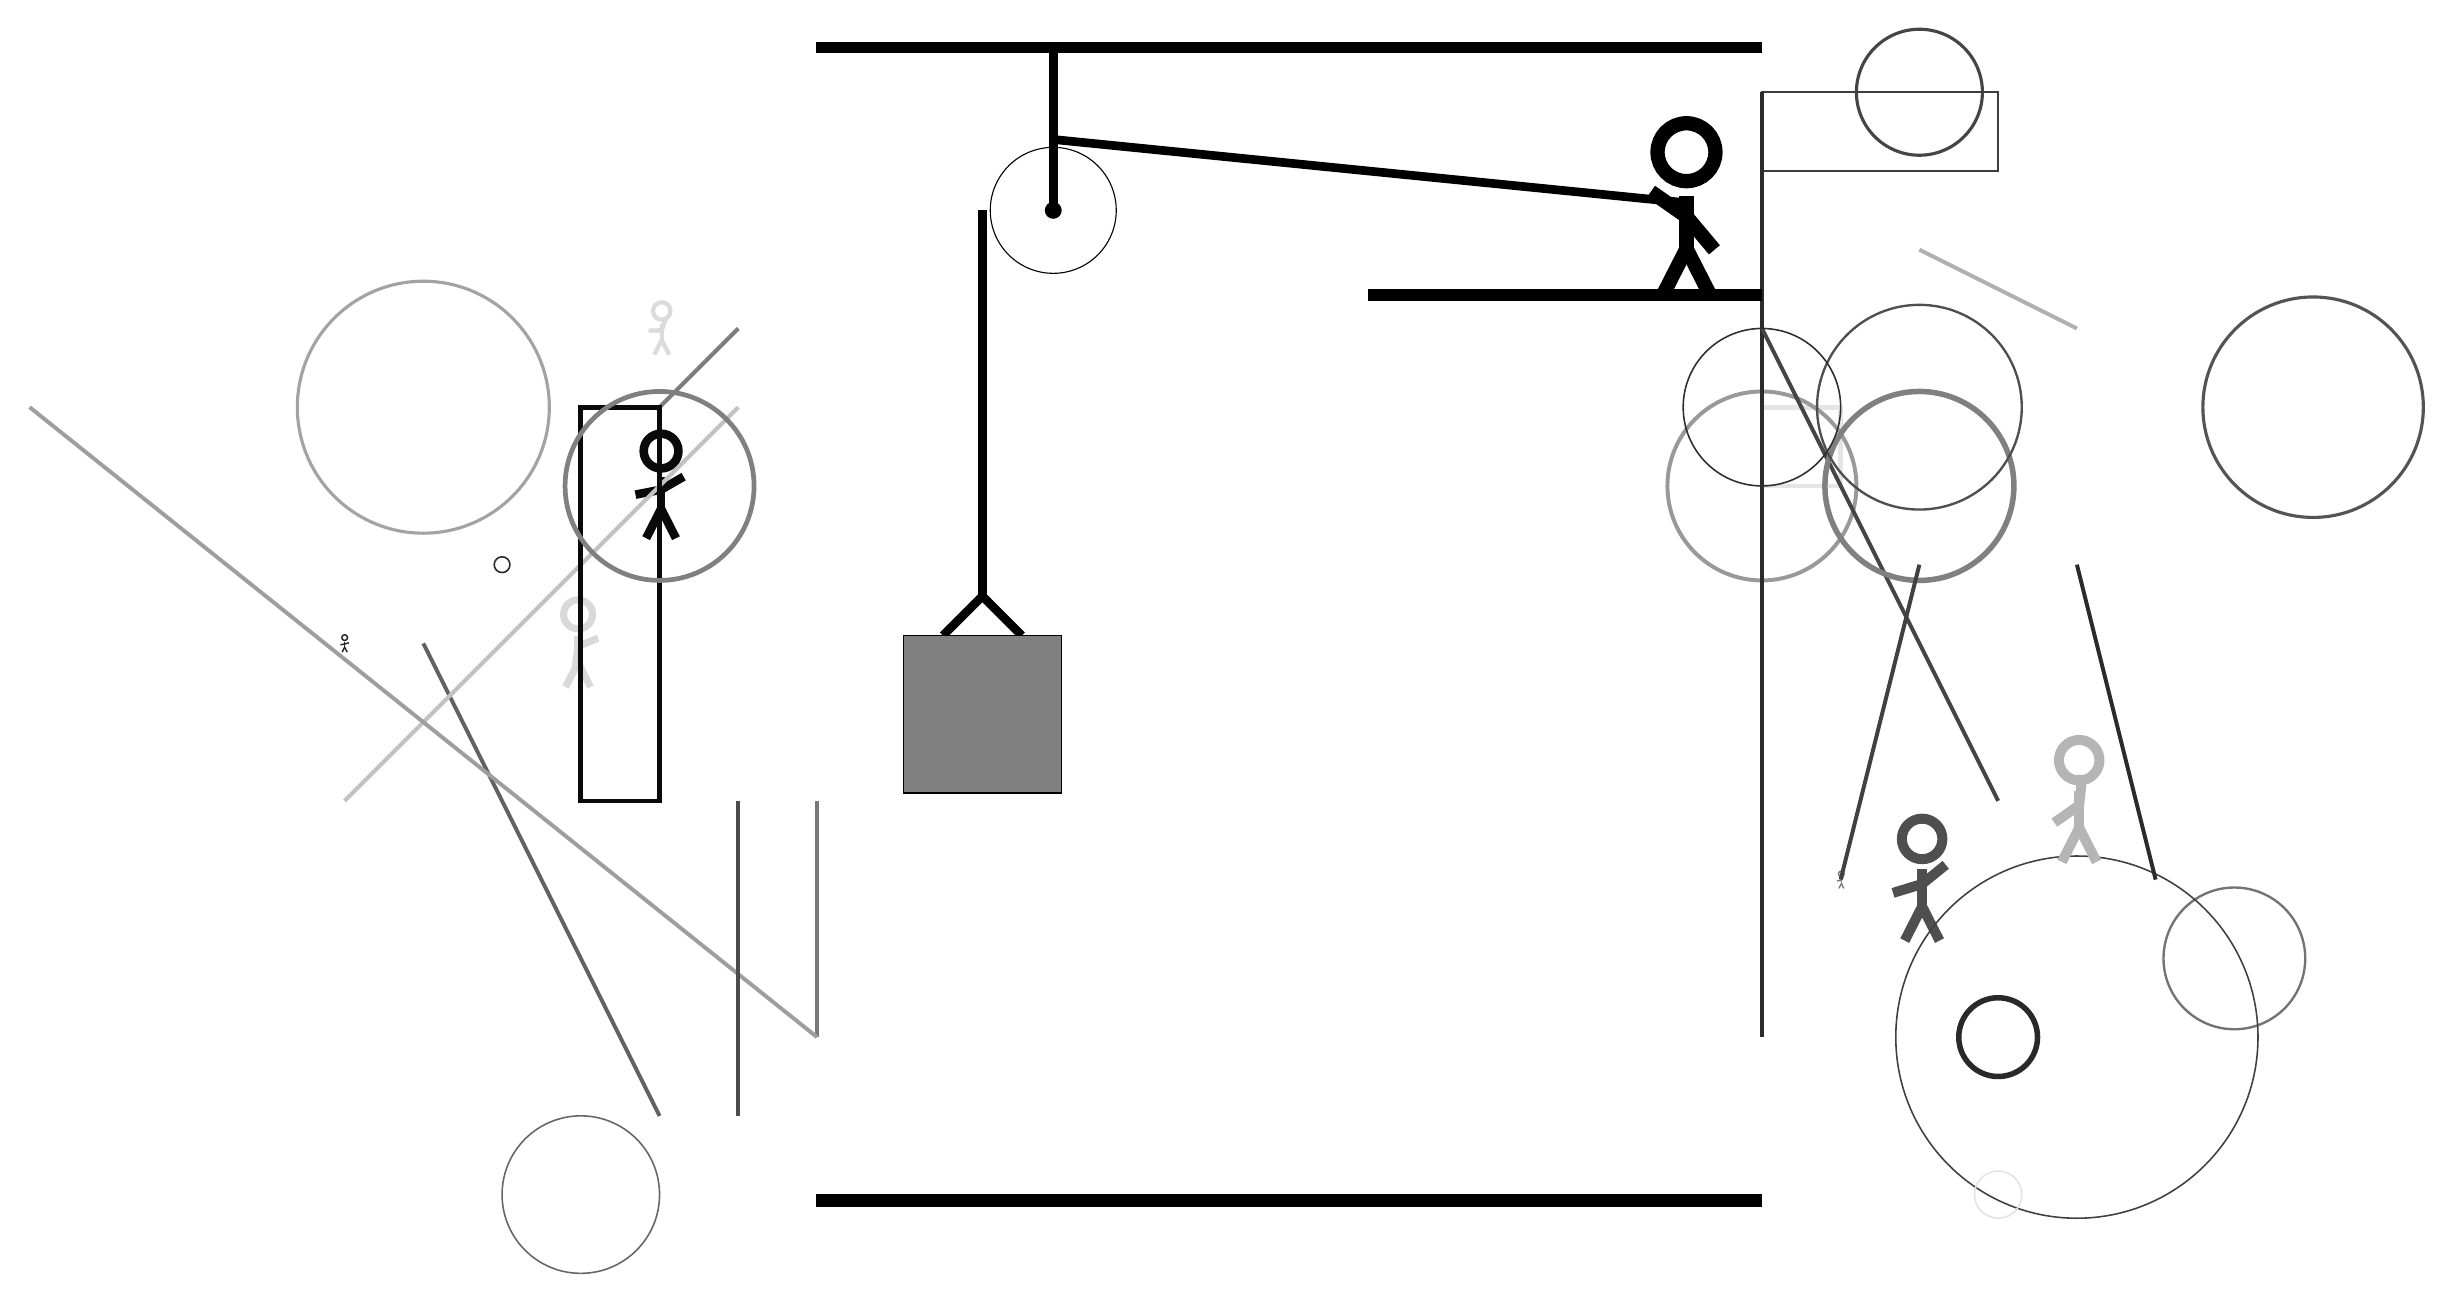
\begin{tikzpicture}
			%%%%% START %%%%%
			
			\draw[fill=black] (-2, 11.5) rectangle (10, 11.625);
			
			\draw (1, 9.5) circle (0.8);
			\draw[fill=black] (1, 9.5) circle (0.1);
			\draw[line width=1.1mm] (1, 11.5) -- (1, 9.5);
			
			\node[line width=0.2mm, color=black!69] at (12, 1) {\Strichmaxerl[7][17][39]};
			
			\draw [line width=0.3mm, color=black!55](16, 0) circle (0.9);
			\node[line width=0.4mm, color=black!14] at (-4, 8) {\Strichmaxerl[3][1][71]};
			\node[line width=0.2mm, color=black!51] at (11, 1) {\Strichmaxerl[1][9][61]};
			\draw[line width=0.5mm, color=black!62](-4, -2) -- (-7, 4);
			\draw[line width=0.5mm, color=black!51](-3, 8) -- (-4, 7);
			\node[line width=0.3mm, color=black!96] at (-4, 6) {\Strichmaxerl[6][11][30]};
			\draw[line width=0.5mm, color=black!53](-2, -1) -- (-2, 2);
			\node[line width=0.2mm, color=black!15] at (-5, 4) {\Strichmaxerl[5][82][23]};
			\draw[line width=0.6mm, color=black!10] (10, 6) rectangle (11, 7);
			\draw [line width=0.4mm, color=black!73](12, 11) circle (0.8);
			\draw[line width=0.5mm, color=black!31](14, 8) -- (12, 9);
			\draw [line width=0.4mm, color=black!67](17, 7) circle (1.4);
			
			\draw [line width=0.2mm, color=black!75](14, -1) circle (2.3);
			\draw[line width=0.5mm, color=black!24](-3, 7) -- (-8, 2);
			\draw [line width=0.5mm, color=black!40](10, 6) circle (1.2);
			
			\draw[line width=0.5mm, color=black!83](14, 5) -- (15, 1);
			\draw [line width=0.2mm, color=black!11](13, -3) circle (0.3);
			\draw[line width=0.2mm, color=black!76] (10, 10) rectangle (13, 11);
			
			\draw [line width=0.4mm, color=black!36](-7, 7) circle (1.6);
			\draw[line width=0.5mm, color=black!83](10, -1) -- (10, 11);
			\draw[line width=0.5mm, color=black!38](-2, -1) -- (-12, 7);
			\draw[line width=0.5mm, color=black!73](10, 8) -- (13, 2);
			\draw [line width=0.7mm, color=black!50](12, 6) circle (1.2);
			\draw [line width=0.7mm, color=black!84](13, -1) circle (0.5);
			\draw [line width=0.3mm, color=black!69](12, 7) circle (1.3);
			\draw [line width=0.2mm, color=black!60](-5, -3) circle (1.0);
			\draw[line width=0.5mm, color=black!75](12, 5) -- (11, 1);
			\draw[line width=0.5mm, color=black!70](-3, 2) -- (-3, -2);
			
			\draw[line width=0.6mm, color=black!96] (-4, 7) rectangle (-5, 2);
			\node[line width=0.5mm, color=black!87] at (-8, 4) {\Strichmaxerl[1][9][17]};
			
			\node[line width=0.6mm, color=black!29] at (14, 2) {\Strichmaxerl[7][35][84]};
			\draw [line width=0.6mm, color=black!50](-4, 6) circle (1.2);
			\draw [line width=0.2mm, color=black!84](-6, 5) circle (0.1);
			
			\draw [line width=0.2mm, color=black!82](10, 7) circle (1.0);
			
			\draw[line width=1.1mm](-0.4, 4.1) --  (0.1, 4.6) -- (0.6, 4.1);
			\draw[fill=black!50] (-0.9, 4.1) rectangle (1.1, 2.1);
			
			\draw[line width=1.1mm](0.1, 9.5) -- (0.1, 4.6);
			\centerarc[line width=1.1mm](1, 9.5)(90:180:0.9)
			\draw[line width=1.1mm](1, 10.4) -- (9, 9.6);
			
			\node at (9, 9.5) {\Strichmaxerl[10][-35][-50]};
			\draw[fill=black] (5, 8.5) rectangle (10, 8.35);
			
			\draw[fill=black] (-2, -3) rectangle (10, -3.15);
			
			%%%%% END %%%%%
		\end{tikzpicture}
	\end{figure}	
\end{document}